%%%% Paramétrage du TD %%%%
\def\xxactivite{Application 1 \ifprof -- Corrigé \else \fi} % \normalsize \vspace{-.4cm}
\def\xxauteur{\textsl{Xavier Pessoles}}


\def\xxnumchapitre{Chapitre 1 \vspace{.2cm}}
\def\xxchapitre{\hspace{.12cm} Correction des systèmes}


\def\xxcompetences{%
\vspace{-.4cm}
\textsl{%
\textbf{Savoirs et compétences :}\\ \vspace{-.4cm}
\begin{itemize}[label=\ding{112},font=\color{ocre}] 
%\item \textit{Res1.C4 : } correction;
\item \textit{Res1.C4.SF1 : } proposer la démarche de réglage d’un correcteur proportionnel, proportionnel intégral et à avance de phase.
%\item \textit{Con.C2 : } 	correction d’un système asservi	;
%\item \textit{Con.C2.SF1 : } choisir un type de correcteur adapté.
\end{itemize}
}}



\def\xxfigures{
%\includegraphics[width=.7\textwidth]{image1}
}%figues de la page de garde

\def\xxtitreexo{Réglage de correcteurs P}
\def\xxsourceexo{\hspace{.2cm} Etude d'un poste de palettisation de bidons. CCPM MP 2010.}

\input{\repRel/Style/pagegarde_TD}
\setcounter{numques}{0}
\setlength{\columnseprule}{.1pt}

\pagestyle{fancy}
\thispagestyle{plain}

\vspace{4.5cm}

\def\columnseprulecolor{\color{ocre}}
\setlength{\columnseprule}{0.4pt} 

%%%%%%%%%%%%%%%%%%%%%%%



\begin{multicols}{2}
\setcounter{exo}{0}

La boucle de position est représentée figure ci-dessous. On admet que : 
\begin{itemize}
\item $H(p)=\dfrac{\Omega_m(p)}{U_v(p)}=\dfrac{30}{1+5\cdot 10^{-3} p}$;
\item $K_r = \SI{4}{V.rad^{-1}}$ : gain du capteur de position;
\item $K_a$ : gain de l'adaptateur du signal de consigne $\alpha_e(t)$;
\item le signal de consigne $\alpha_e(t)$ est exprimé en degrés;
\item le correcteur $C(p)$ est à action proportionnelle de gain réglable $K_c$.
\end{itemize}

\begin{obj}
\begin{itemize}
\item On souhaite une marge de phase de 45\degres.
\item On souhaite un écart de traînage inférieur à 1\degres pour une consigne de vitesse de \SI{105}{\degres.s^{-1}}. 
\end{itemize}
\end{obj}

\begin{center}
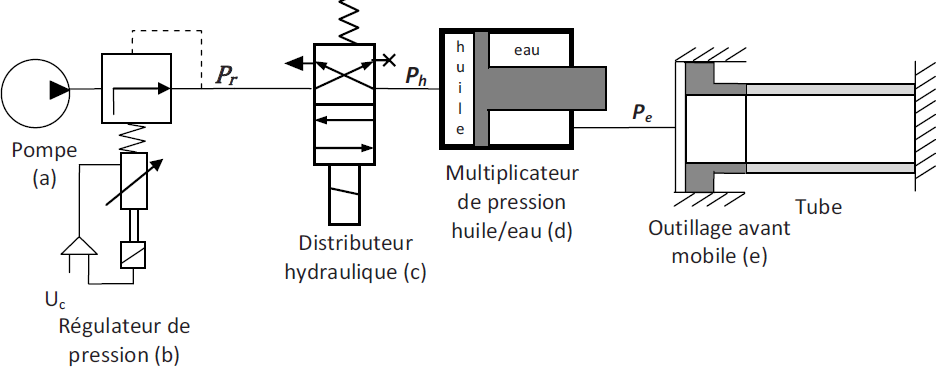
\includegraphics[width=\linewidth]{fig_01}
\end{center}

\question{Déterminer la fonctionde transfert $R(p)= \dfrac{\alpha_r(p)}{\Omega_m(p)}$ du réducteur.}
\ifprof
\begin{corrige}

\end{corrige}
\else
\fi


\question{Déterminer le gain $K_a$ de l'adaptateur.}
\ifprof
\begin{corrige}

\end{corrige}
\else
\fi


\question{Déterminer, en fonction notamment de $K_m'$ et $t_m'$, la fonction de transfert
en boucle ouverte $T(p)$ que l’on exprimera sous forme canonique. En déduire l’expression du
gain de boucle, noté $K_{\text{BO}}$. }
\ifprof
\begin{corrige}

\end{corrige}
\else
\fi

On souhaite une marge de phase de 45\degres.

\question{Déterminer la valeur de $K_{\text{BO}}$ permettant de satisfaire cette condition.}
\ifprof
\begin{corrige}

\end{corrige}
\else
\fi



\question{En déduire la valeur du gain $K_c$ du correcteur. }
\ifprof
\begin{corrige}

\end{corrige}
\else
\fi



\question{Déterminer l’écart de position. Conclure vis-à-vis des exigences du cahier des
charges. }
\ifprof
\begin{corrige}

\end{corrige}
\else
\fi

On souhaite un écart de traînage inférieur à 1\degres pour une consigne de vitesse de \SI{105}{\degres.s^{-1}}. 

\question{Déterminer l’expression de $\alpha_e(t)$ correspondant à une consigne de vitesse
de \SI{105}{\degres.s^{-1}}. En déduire $\alpha_e(p)$.}
\ifprof
\begin{corrige}

\end{corrige}
\else
\fi


\question{La valeur de $K_{\text{BO}}$ définie précédemment permet-elle de satisfaire l’exigence
de précision imposée par le cahier des charges ? Conclure. }
\ifprof
\begin{corrige}

\end{corrige}
\else
\fi



\end{multicols}
